\documentclass{article}
\usepackage{graphicx}
\usepackage{Sweave}
\usepackage{amsmath}
\usepackage[margin=1in]{geometry}
\usepackage{booktabs} 

\title{Integración en la UE: Resultados}
\author{Alba Nuez Vilà}
\date{Julio 2024}

\Sconcordance{concordance:Informe_resultados.tex:Informe_resultados.Rnw:1 30 1 1 27 1 %
2 8 1}


\begin{document}
\maketitle

\section{Actitud hacia los demás e inmigración}

\begin{center}
\emph{¿Cómo varía la actitud hacia los demás en diferentes países de la UE? ¿Cómo se correlaciona con la percepción del bienestar en relación con la inmigración?}
\end{center}

Las actitudes sociales y la percepción sobre la inmigración se influencian mutuamente. Entender cómo se dan estas relaciones puede ser crucial para mejorar la cohesión social y formular políticas de integración efectivas.

La variable ``actitud hacia los demás'' se obtiene calculando el promedio de las variables ``confianza'', ``honestidad'' y ``ayuda'', como puede observarse en la siguiente fórmula...

\[
\text{actitud hacia los demás} = \frac{\text{confianza} + \text{honestidad} + \text{ayuda}}{3}
\]

Estas variables están codificadas en una escala Likert, presentan patrones de respuesta similares y abordan cuestiones relacionadas (\textit{ver más detalle en el documento de planificación}). Esta variable varía de 0 a 10, donde 0 indica una actitud muy negativa hacia los demás y 10 una actitud muy positiva.

A nivel europeo, la distribución de esta variable muestra que la mayoría de encuestados presentan una actitud positiva hacia los demás, con una clara tendencia a valores superiores a 5.

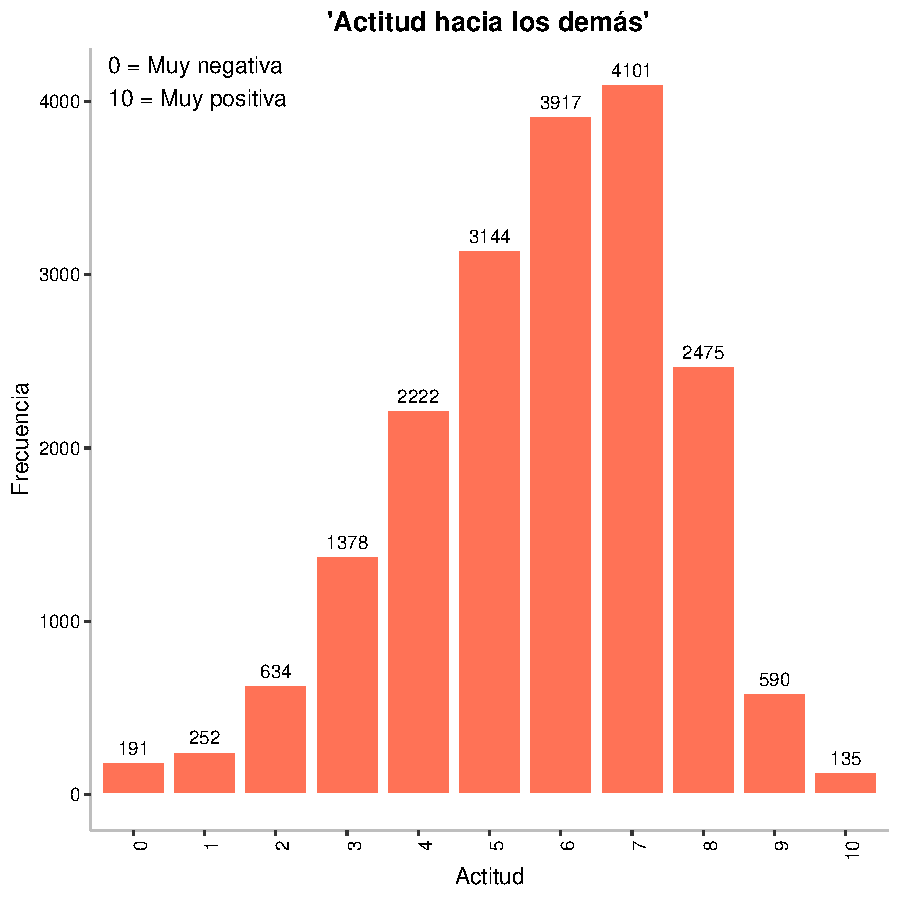
\includegraphics{Informe_resultados-histogram}


La actitud hacia los demás parece estar fuertemente influenciada por el país de origen del encuestado. Según el mapa de calor, los encuestados de Eslovaquia (SK) y Hungría (HU) tienden a mostrar una actitud menos favorable hacia los demás, con niveles de confianza, honestidad y ayuda por debajo de 5. En contraste, los encuestados austriacos (AT) muestran una actitud más positiva, con una respuesta predominante de 7 en estas variables.

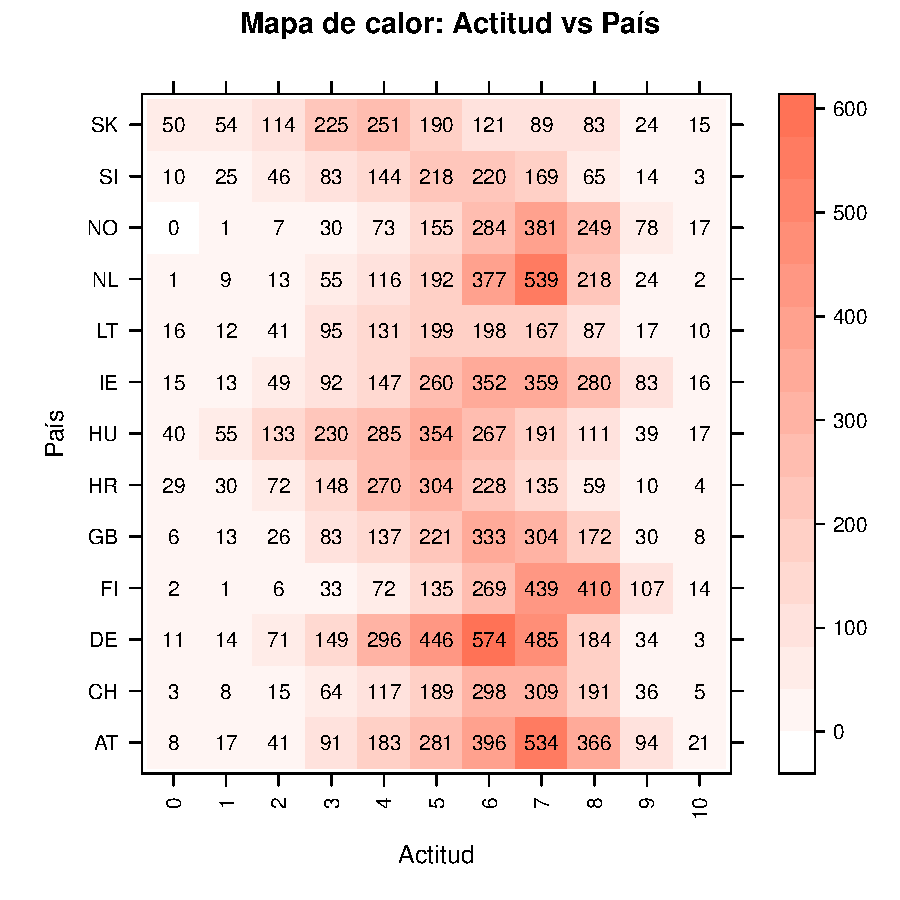
\includegraphics{Informe_resultados-003}

En esta misma línea, los encuestados de Eslovaquia (SK) y Hungría (HU) mayoritariamente opinan que la inmigración es mala para la economía de su país, mientras que los encuestados de Alemania (DE) o Austria (AT) tienden a tener una opinión positiva acerca del impacto de inmigración en la economía.

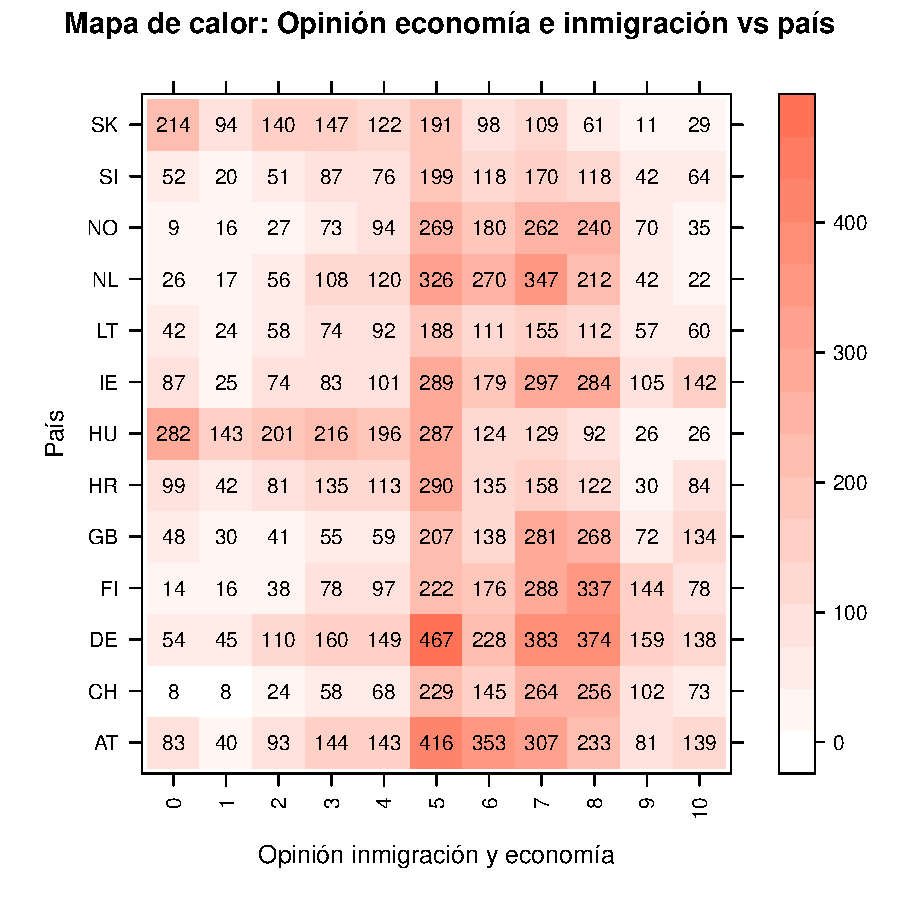
\includegraphics{Informe_resultados-004}

Finalmente, a nivel europeo parece existir una correlación entre la actitud hacia los demás y la opinión acerca del impacto de la inmigración en la calidad de vida, hecho que puede observarse en la marcada diagonal en el mapa de calor:

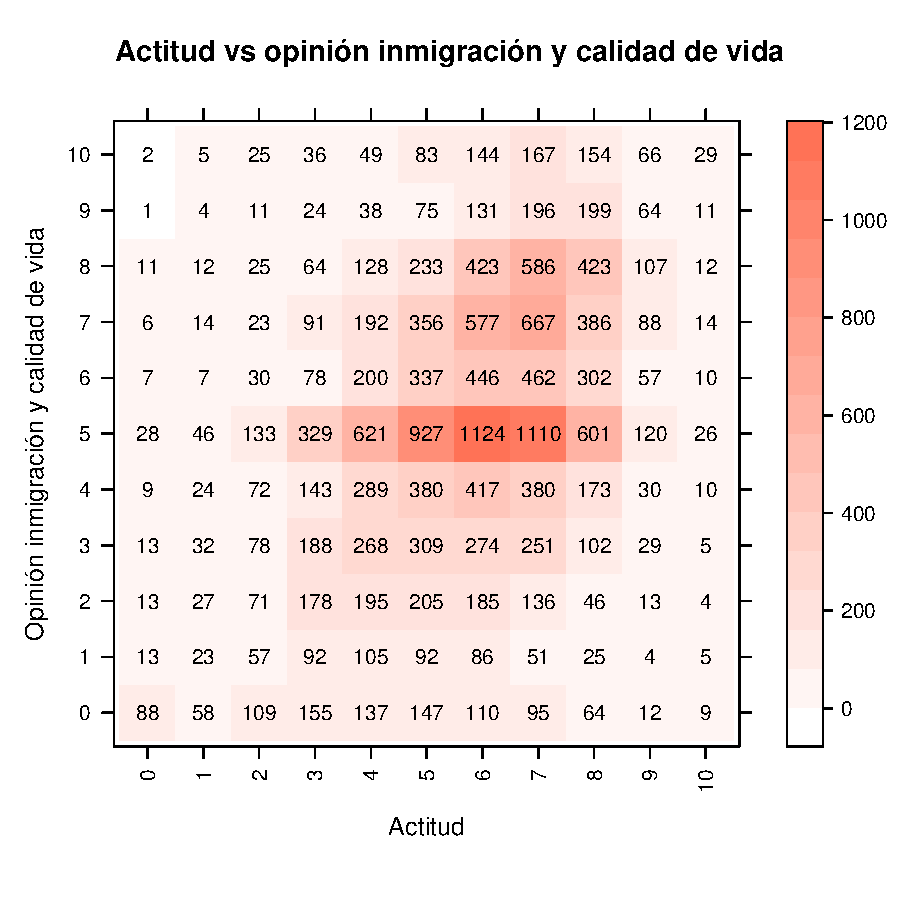
\includegraphics{Informe_resultados-005}




\section{Adopción LGTBQ+}

\begin{center}
\emph{¿Cómo difieren las opiniones sobre la adopción LGTBQ+ entre países?}
\end{center}

Existen notables diferencias en la opinión sobre la adopción por parte de personas homosexuales entre diferentes países. Por ejemplo, Austria (AT), Países Bajos (NL) y Noruega (NO) muestran un fuerte apoyo a este derecho, mientras que Eslovaquia (SK), Lituania (LT), Hungría (HU) y Croacia (HR) están mayoritariamente en contra, como se evidencia en la siguiente tabla (o el gráfico de barras apiladas incluido en el \emph{dashboard}):

\begin{table}[h!]
\centering
\caption{Opinión adopción LGTBQ+ por país (1 = muy a favor, 5 = muy en contra)}
\begin{tabular}{lrrrrrr}
\toprule
\textbf{País} & \textbf{1} & \textbf{2} & \textbf{3} & \textbf{4} & \textbf{5} & \textbf{NS/NC} \\
\midrule
AT & 621 & \textbf{748} & 436 & 273 & 162 & 114 \\
CH & 326 & \textbf{434} & 236 & 223 & 129 & 36 \\
DE & \textbf{935} & 881 & 235 & 215 & 117 & 37 \\
FI & \textbf{560} & 470 & 216 & 194 & 94 & 29 \\
GB & \textbf{618} & 562 & 218 & 148 & 81 & 57 \\
HR & 89 & 267 & 229 & \textbf{492} & 409 & 77 \\
HU & 161 & 388 & \textbf{540} & 432 & 527 & 70 \\
IE & \textbf{734} & 586 & 326 & 148 & 145 & 78 \\
LT & 26 & 136 & 237 & \textbf{490} & 449 & 27 \\
NL & \textbf{882} & 497 & 145 & 90 & 62 & 19 \\
NO & \textbf{622} & 395 & 172 & 89 & 52 & 7 \\
SI & 128 & 349 & 208 & \textbf{289} & 224 & 50 \\
SK & 36 & 155 & 243 & 329 & \textbf{610} & 69 \\
\bottomrule
\end{tabular}
\end{table}
\end{document}
